\documentclass{standalone}
\usepackage{tikz}
\usepackage{ctex,siunitx}
\setCJKmainfont{Noto Serif CJK SC}
\usepackage{tkz-euclide}
\usepackage{amsmath}
\usetikzlibrary{patterns, calc}
\usetikzlibrary {decorations.pathmorphing, decorations.pathreplacing, decorations.shapes,}

\begin{document}
\small
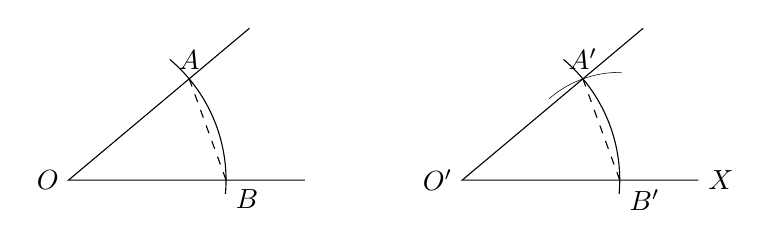
\begin{tikzpicture}[>=stealth,scale=1]
  \tkzSetUpPoint[fill=black]
  % \useasboundingbox(-1,-0.75)rectangle(3.7,1.4);
\begin{scope}
\draw(40:3)--(0,0)node[left]{$O$}--(3,0);
\draw(-5:2) arc (-5:50:2);
\node at (40:2)[above]{$A$};
\draw[dashed](2,0)node[below right]{$B$}--(40:2);
\end{scope}
\begin{scope}[xshift=5cm]
	\draw(40:3)--(0,0)node[left]{$O'$}--(3,0)node[right]{$X$};
	\draw(-5:2) arc (-5:50:2);
	\node at (40:2)[above]{$A'$};
	\draw[dashed](2,0)node[below right]{$B'$}--(40:2);
\tkzDefPoint(2,0){B'}
\tkzDefPoint(40:2){A'}
\tkzCompass[color=black](B',A')
\end{scope}
\end{tikzpicture}
\end{document}